
%(BEGIN_QUESTION)
% Copyright 2006, Tony R. Kuphaldt, released under the Creative Commons Attribution License (v 1.0)
% This means you may do almost anything with this work of mine, so long as you give me proper credit

Spenning og strøm er relatert til hverandre gjennom {\it integralfunksjoner} når vi arbeider med kondensatorer og induktorer. I motsetning til motstander, der spenning og strøm følger hverandre i direkte proporsjon, introduserer kondensatorer og induktorer en tredje variabel, {\it tid}, i relasjonene mellom spenning og strøm.

Bestem hvilken variabel som er integralet av hvilken, for hver av disse kretsene, ved å plotte begge variabler over tid. Skriv deretter et kalkulusuttrykk for hver krets som viser de respektive sammenhengene mellom spenning og strøm. Anta {\it perfekte} kondensatorer og induktorer, uten intern motstand eller andre ikke-ideelle egenskaper:
 
$$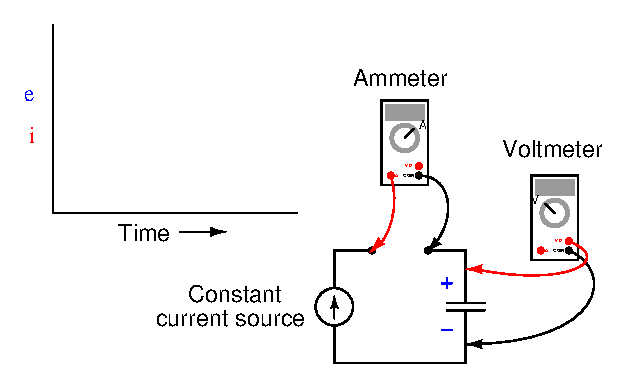
\includegraphics[width=15.5cm]{i01569x01.eps}$$

$$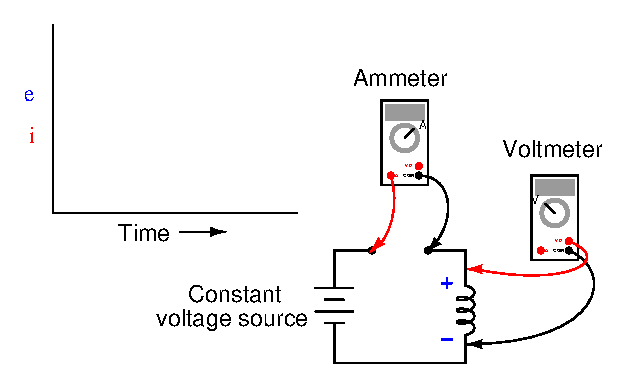
\includegraphics[width=15.5cm]{i01569x02.eps}$$

Hint: husk disse ligningene, som tilsvarer Ohms lov for kondensatorer og induktorer:

$$i = C {dv \over dt}$$

$$v = L {di \over dt}$$

\underbar{file i01569}
%(END_QUESTION)





%(BEGIN_ANSWER)

$$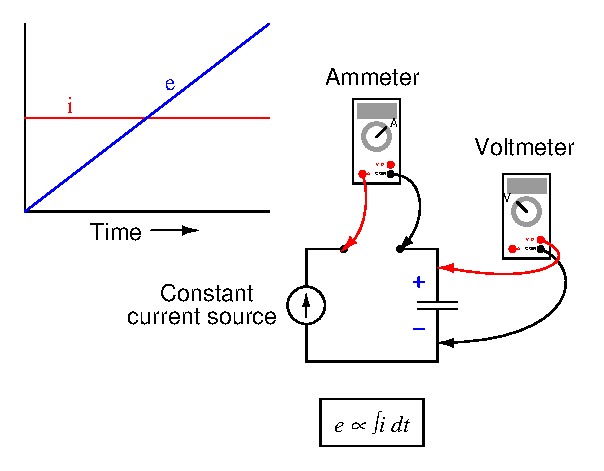
\includegraphics[width=15.5cm]{i01569x03.eps}$$

$$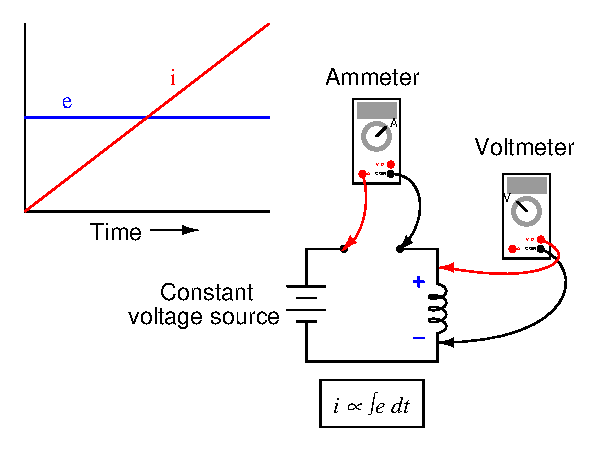
\includegraphics[width=15.5cm]{i01569x04.eps}$$

%(END_ANSWER)





%(BEGIN_NOTES)



%INDEX% Mathematics, calculus: derivative vs integral (applied to capacitors and inductors)

%(END_NOTES)

